\documentclass{article}
\usepackage{fullpage}
\usepackage[utf8]{inputenc}
\usepackage[T1, T2A]{fontenc}
\usepackage[english, russian]{babel}
\usepackage{indentfirst}
\usepackage{graphicx}
\selectlanguage{russian}
\graphicspath{{./graphics/}}

\begin{document}
\begin{titlepage}
    \begin{center}
        \normalsize
        МГТУ им Н.Э. Баумана, кафедра ИУ5 \\
        \vspace*{1cm}
        \LARGE
        \textbf{Лабораторная работа №1 по дисцилине "РИП"}

        \vspace{0.5cm}
    \end{center}
    \vfill

    \begin{flushright}
        \textbf{Выполнил:} Никольский Даниил, ИУ5-51б \\
        \textbf{Проверил:} Гапанюк Юрий Евгеньевич, ИУ5 \\
    \end{flushright}
    \vspace{1.5cm}
    \begin{flushleft}
        \textbf{Дата: \today} \\
        \textbf{Подпись: Никольский Д.Р.} \\
    \end{flushleft}
\end{titlepage}

\tableofcontents
\newpage
\section{Задание}
В этой лабораторной работе необходимо составить MindMap и концептуальную карту по теме проекта домашнего задания №2.
\begin{enumerate}
    \item MindMap используется для описания организационных структур или простых вариантов сущностей предметной области. Для выполнения этой части задания можно использовать пакет XMind или сервис MindMup.

    \item Концептуальные карты используются для описания сложных вариантов сущностей предметной области с учетом связей между ними. Для выполнения этой части задания можно использовать пакет CmapTools.

\end{enumerate}
В результате выполнения домашнего задания должны быть разработаны MindMap и концептуальная карта.

\section{Краткое описание предметной области}
В системе «Банк вкладов» клиенты могут просматривать доступные условия вкладов и составлять наиболее выгодный для себя вариант вклада, установив такие параметры, как срок (есть несколько зафиксированных вариантов срока вклада со своим типом начисления процентов – ежемесячно или ежегодно), сумма (в рублях или иностранной валюте на выбор из доступных), тип вклада (пополняемый, непополняемый, с возможностью снятия средств или без и т.д.). После выбора условий вклада клиент резервирует время обслуживания в отделении, где сотрудник данного отделения оформляет нового клиента и вклад (в случае отсутствия у него карты банка) – вносит его ФИО, паспортные данные, телефон и связывает их с номером карты, или сразу оформляет вклад.

\newpage
\section{Mindmap}
\begin{figure}[!h]
    \centering
    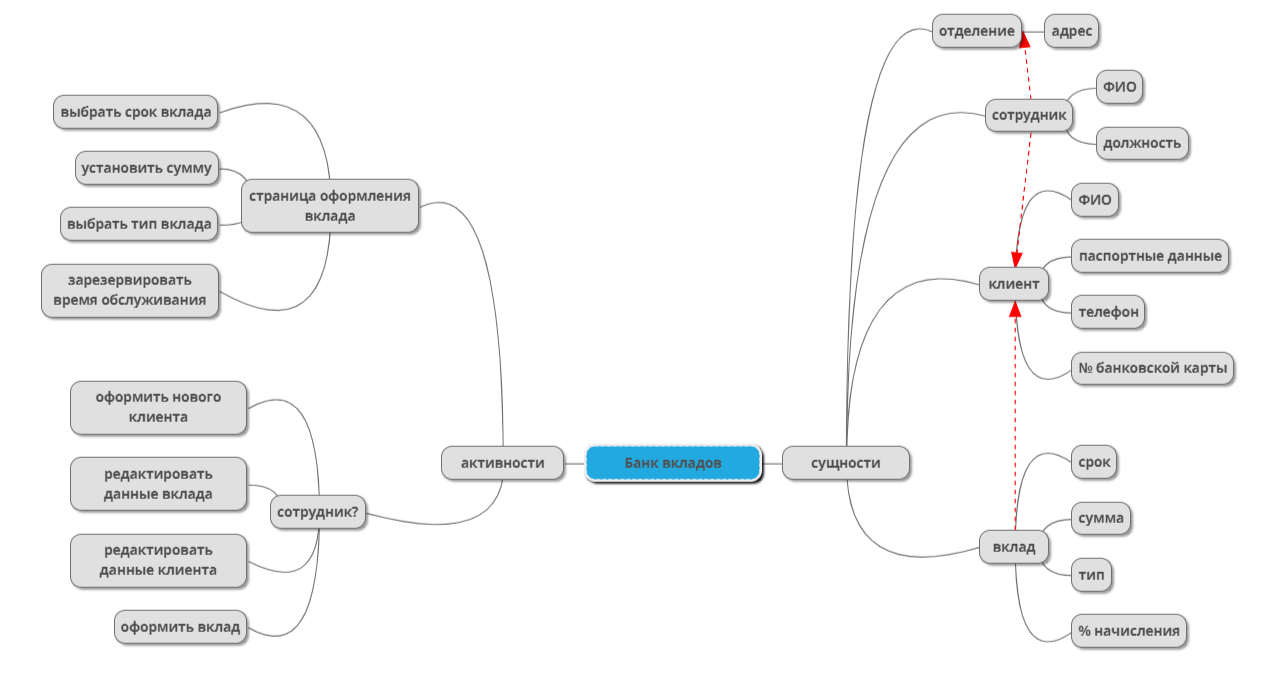
\includegraphics[width=\textwidth]{mindmap.png}
    \caption{Mindmap}
\end{figure}

\newpage
\section{Концептуальная карта}
\begin{figure}[!h]
    \centering
    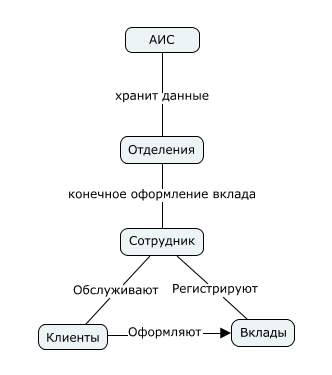
\includegraphics{concept_map.png}
    \caption{Концептуальная карта}
\end{figure}

\end{document}